% !TEX encoding = UTF-8
\documentclass[a4paper,12pt]{article}
\usepackage[T1]{fontenc}
\usepackage[utf8]{inputenc}
\usepackage[italian]{babel}
\usepackage{color, colortbl}
\usepackage{graphicx}
\definecolor{Ash}{rgb}{0.7,0.75,0.71}
\usepackage{multirow}
\usepackage{float}



\begin{document}

\title{\textbf{TrackMyCar - Live Positioning System} \\ Test Plan}

\author{Kevin Mansoldo, Matteo Dal Monte, Luca Vicentini}
\date{30 Giugno 2015}
\maketitle
\pagebreak

\tableofcontents
\pagebreak

\section{Lista Destinatari del Documento}

\begin{table*}[ht]
\begin{center}
\begin{tabular}{p{1cm} p{4.5cm} p{3.5cm} p{3.5cm}}
\rowcolor{Ash}
\hline
Copia & Persona & Organizzazione & 30 Giugno 2015 \\ \hline
1 & Kevin Mansoldo & Azienda & 30 Giugno 2015 \\ 
2 & Matteo Dal Monte & Azienda & 30 Giugno 2015 \\ 
3 & Luca Vicentini & Azienda & 30 Giugno 2015 \\ 
4 & Claudio Tomazzoli & Cliente & 30 Giugno 2015 \\ \hline
\end{tabular}
\end{center}


\begin{center}
\begin{tabular}{p{6cm} p{3.5cm} p{3.5cm}}
\rowcolor{Ash}
\hline
Azione & Persona & Data \\ \hline
Documento redatto da & Kevin Mansoldo & 30 Giugno 2015 \\ 
Documento approvato da & Matteo Dal Monte & 30 Giugno 2015 \\ 
Documento approvato da & Luca Vicentini & 30 Giugno 2015 \\ \hline
\end{tabular}
\end{center}
\end{table*}

\subsection{Versione Documento}
\begin{table*}[ht]
\begin{center}
\begin{tabular}{p{1cm} p{3cm} p{5cm} p{3.5cm}}
\rowcolor{Ash}
\hline
Versione & Autore & Note & Data \\ \hline
1.0 & Kevin Mansoldo & Stesura Iniziale & 8 Giugno 2015 \\ 
1.1 & Kevin Mansoldo & Revisione su osservazioni del gruppo & 17 Giugno 2015 \\ 
1.2 & Kevin Mansoldo & Revisione Finale & 30 Giugno 2015 \\ \hline
\end{tabular}
\end{center}
\end{table*}

\subsection{Supporto Documento}
\begin{table*}[ht]
\begin{center}
\begin{tabular}{p{6cm} p{5cm} p{2cm}}
\rowcolor{Ash}
\hline
Nome File & Tipo & Estensione \\ \hline
TestPlan & Portable Document Format & .pdf \\ \hline
\end{tabular}
\end{center}
\end{table*}

\clearpage

\pagebreak

\section{Introduzione e Obiettivi}

Lo scopo del sistema che si vuole implementare è quello di poter tracciare in tempo reale il o i veicoli collegati in caso di furto o smarrimento. Tramite un'interfaccia visuale è possibile tenere sotto controllo la posizione, la velocità e lo storico dei percorsi effettuati. Inoltre viene fornita la possibilità di sfruttare l'integrazione con sistemi di videosorveglianza interni al veicolo, identificando così eventuali malintenzionati. 

L'applicazione, dotata di una intuitiva interfaccia grafica, permette quindi la rapida fruizione dei contenuti tramite semplici menu contestuali.


\section{Definizioni, Acronimi e Abbreviazioni}

Per le definizioni di alcuni termini fondamentali, fare riferimento al glossario ``Glossario.pdf'' all'interno della documentazione di progetto.

\begin{table}[h]
\begin{center}
\begin{tabular}{ p{4.5cm} p{4.5cm} p{3.5cm} } 
\rowcolor{Ash}	
\hline	
Nome File & Tipo File & Estensione  \\ \hline
Development Case & Linee guida di sviluppo del progetto & DevCase.pdf  \\ 
Glossario & Descrizione di termini specifici & Glossario.pdf  \\ 
Vision & Requisiti di sistema, Business Needs e Motivazioni & Vision.pdf  \\ 
Caratteristiche & Requisiti funzionali, non funzionali ed architetturali & Caratteristiche.pdf  \\ \hline
\end{tabular}
\end{center}
\end{table}

\pagebreak

\section{Test Plan}
Pianificazione dei test di ogni iterazione che include elenco attività, calendario e risorse coinvolte (Gantt)
\begin{figure}[ht]
\centering
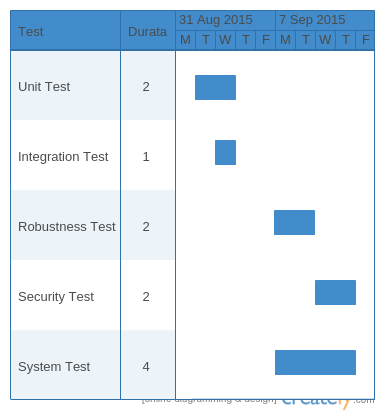
\includegraphics[trim={0 0.5cm 0 0}, clip, scale=0.5]{test.png}
\end{figure}

\section{Tipologia Test}
Divideremo i test in due grandi famiglie
\begin{itemize}	

\item White Box (test Strutturali):
\begin{itemize}	

\item Unit Test;
\item Integration Test;
\item System Test.

\end{itemize}

\item Black Box (test Funzionali).

\begin{itemize}	

\item Funzioni Amministratore;
\item Funzioni Utente.
\item Funzioni comuni.

\end{itemize}

\end{itemize}

\subsection{White Box (test Strutturali)}
\subsubsection{Unit Test}
\textbf{Tester:} Kevin Mansoldo\\
\textbf{Data:} 1/9/2015\\
\textbf{Tipo:} automatico\\
\textbf{Oggetto:} Package univr.is.tmc.test\\
\textbf{Prerequisiti:} Nessuno\\
\textbf{Applicazioni necessarie:} JUnit\\
\textbf{Breve descrizione:} Test sul corretto funzionamento delle classi responsabili del controllo della velocità  rispetto al limite impostato ed eventuale soglia di superamento di quest'ultimo.\\ \\

Test effettuati:
\begin{enumerate}
\item RispettaLimite : controlla se la velocità è compresa nell'intervallo min\_limite e max\_limite.
\item SuperaLimite : controlla la soglia di superamento del limite rispetto alla velocità inserita.
\end{enumerate}



\begin{table}[ht]
\begin{center}
\begin{tabular}{p{1cm} p{3cm} p{3cm} p{3cm} p{2cm}}
\rowcolor{Ash}
\hline
\# & Limite & Velocità & Risultato Atteso & Esito \\ \hline
1 & 0-130 & 100 & true & \cellcolor{green}{OK}\\
2 & 0-130 & 145 & 15 & \cellcolor{green}{OK}\\ \hline
\end{tabular}
\end{center}
\end{table}

\pagebreak

\subsubsection{Integration Test}
\textbf{Tester:} Matteo Dal Monte\\
\textbf{Data:} 2/9/2015\\
\textbf{Oggetto:} TrackMyCar\\
\textbf{Prerequisiti:} Base di dati, applicazione web, simulatore SW\\
\textbf{Applicazioni necessarie:} Browser\\
\textbf{Breve descrizione:} Si è testata l'integrazione tra i vari componenti del sistema TMC: il simulatore SW (Modulo HW), la web application (pagine jsp), le Servlet e il DB.\\

\pagebreak

\subsubsection{System Test}
\textbf{Tester:} Kevin Mansoldo\\
\textbf{Data:} 7/9/2015\\
\textbf{Oggetto:} WebApp\\
\textbf{Prerequisiti:} Webapp\\
\textbf{Applicazioni necessarie:} Browser\\
\textbf{Breve descrizione:} I test in questa sezione ci hanno permesso di controllare alcune proprietà  del nostro sistema.\\

\begin{itemize}	

\item Robustness Test:
Il nostro sistema controlla la validità dei campi inseriti prima della loro modifica/inserimento nel sistema.
Nel caso i dati inseriti fossero scorretti, il sistema reindirizza l'utente ad una pagina di errore notificando il fatto con un messaggio di errore indicando la natura dello stesso; nel caso, invece, di mancata compilazione dei campi non è possibile proseguire nell'operazione scelta notificando il motivo (es. mail mancante).
\item Security Test:
\begin{table}[ht]
\begin{center}
\begin{tabular}{p{6.5cm} | p{6.5cm}}
\rowcolor{Ash}
\hline
Azione & Conseguenza \\ \hline
Controllo sessione pagina & reindirizzamento Login. \\
\vspace{0.2cm}\\
Controllo permessi pagina & vengono visualizzate solo le operazioni disponibili per l'utente loggato. \\
\vspace{0.2cm}\\
Tentativo accesso tramite URL da parte di utenti non autorizzati & reindirizzamento Login. \\ \hline
\end{tabular}
\end{center}
\end{table}

\end{itemize}

\pagebreak

\subsection{Black Box (Test Funzionali)}
Si testano i casi d'uso e i requisiti funzionali dell'analisi\\ \\
\textbf{Tester:} Matteo Dal Monte\\
\textbf{Data:} 7/9/2015\\
\textbf{Oggetto:} Webapp\\
\textbf{Prerequisiti:} Webapp\\
\textbf{Applicazioni necessarie:} Browser\\
\textbf{Breve descrizione:} Si testano i casi d'uso e i requisiti funzionali dell'analisi\\

\subsubsection{Funzioni Amministratore}
Test sugli use case legati allo stakeholder Amministratore:

\begin{table}[H]
\begin{center}
\caption{Riepilogo Aree di Test}
\begin{tabular}{l l l l}
\rowcolor{Ash}
\hline
\# & Ambito & Risultato Atteso & Esito \\ \hline
1 & Gestione Utenti				&		gestione utenti corretta				&\cellcolor{green}{OK}\\
2 & Gestione Veicoli				&		gestione veicoli corretta				&\cellcolor{green}{OK}\\
3 & Associazione Utente-Veicolo	&		associazione effettuata con successo	&\cellcolor{green}{OK}\\
4 & Imposta Allarme				&		impostazione effettuata con successo	& \cellcolor{green}{OK}\\ \hline
\end{tabular}
\end{center}
\end{table}

\begin{table}[H]
\begin{center}
\caption{Dettaglio Area di Test \#1}
\begin{tabular}{p{0.5cm} p{6.5cm} p{5cm} p{1cm}}
\rowcolor{Ash}
\hline
\# & Azione & Risultato Atteso & Esito \\ \hline
1 & Nuovo Utente con email esistente				&		messaggio di errore		&\cellcolor{green}{OK}\\
2 & Nuovo Utente con dati errati					&		messaggio di errore		&\cellcolor{green}{OK}\\
3 & Nuovo Utente con dati corretti					&		inserimento effettuato	&\cellcolor{green}{OK}\\
4 & Selezione Utente, Modifica						&		pagina di modifica		&\cellcolor{green}{OK}\\
5 & Pagina di modifica, dati corretti					&		modifica effettuata		&\cellcolor{green}{OK}\\
6 & Modifica, senza selezione						&		messaggio di errore		&\cellcolor{green}{OK}\\
7 & Selezione utente, Elimina						&		cancellazione effettuata	&\cellcolor{green}{OK}\\
8 & Elimina, senza selezione						&		messaggio di errore		&\cellcolor{green}{OK}\\
9 & Elimina ultimo amministratore					&		messaggio di errore		&\cellcolor{green}{OK}\\ \hline
\end{tabular}{}
\end{center}
\end{table}

\begin{table}[H]
\begin{center}
\caption{Dettaglio Area di Test \#2}
\begin{tabular}{p{0.5cm} p{6.5cm} p{5cm} p{1cm}}
\rowcolor{Ash}
\hline
\# & Azione & Risultato Atteso & Esito \\ \hline
1 & Nuovo Veicolo con targa esistente				&		pagina di errore		&\cellcolor{green}{OK}\\
2 & Nuovo Veicolo con dati errati					&		messaggio di errore		&\cellcolor{green}{OK}\\
3 & Nuovo Veicolo con dati corretti					&		inserimento effettuato	&\cellcolor{green}{OK}\\
4 & Selezione Veicolo, Modifica					&		pagina di modifica		&\cellcolor{green}{OK}\\
5 & Pagina di modifica, dati corretti					&		modifica effettuata		&\cellcolor{green}{OK}\\
6 & Modifica, senza selezione						&		messaggio di errore		&\cellcolor{green}{OK}\\
7 & Selezione Veicolo, Elimina						&		cancellazione effettuata	&\cellcolor{green}{OK}\\
8 & Elimina, senza selezione						&		messaggio di errore		&\cellcolor{green}{OK}\\ \hline
\end{tabular}
\end{center}
\end{table}

\begin{table}[H]
\begin{center}
\caption{Dettaglio Area di Test \#3}
\begin{tabular}{p{0.5cm} p{7cm} p{4.5cm} p{1cm}}
\rowcolor{Ash}
\hline
\# & Azione & Risultato Atteso & Esito \\ \hline
1 & Associazione Utente-Veicolo esistente			&		messaggio di errore		&\cellcolor{green}{OK}\\
2 & Inserisci, senza selezione						&		messaggio di errore		&\cellcolor{green}{OK}\\
3 & Selezione Utente, Veicolo, inserisci				&		inserimento effettuato	&\cellcolor{green}{OK}\\
4 & Elimina senza selezione						&		messaggio di errore		&\cellcolor{green}{OK}\\
5 & Selezione Utente, Veicolo, Elimina				&		eliminazione effettuata	&\cellcolor{green}{OK}\\
5 & Veicolo e/o Utente non in DB					&		non viene visualizzato	&\cellcolor{green}{OK}\\ \hline
\end{tabular}
\end{center}
\end{table}

\begin{table}[H]
\begin{center}
\caption{Dettaglio Area di Test \#4}
\begin{tabular}{p{0.5cm} p{8cm} p{3.5cm} p{1cm}}
\rowcolor{Ash}
\hline
\# & Azione & Risultato Atteso & Esito \\ \hline
1 & Imposta limite fino a 300 Km/h	&	limite impostato		&	\cellcolor{green}{OK}\\
1 & Imposta limite oltre 300 Km/h	&		messaggio errore	&		\cellcolor{green}{OK}\\ \hline
\end{tabular}
\end{center}
\end{table}

\pagebreak

\subsubsection{Funzioni Regular}

Test sugli use case legati allo stakeholder Regular

\begin{table*}[h]
\begin{center}
\caption{Riepilogo Aree di Test}
\begin{tabular}{p{0.5cm} p{3.8cm} p{7.7cm} p{1cm}}
\rowcolor{Ash}
\hline
\# & Ambito & Risultato Atteso & Esito \\ \hline
1 & Visualizza Posizione	& mappa con posizione dei veicoli associati a utente loggato			& \cellcolor{green}{OK}\\
2 & Live Tracking		& scelta furto corrente e mappa con posizione in tempo reale del veicolo e video & \cellcolor{green}{OK}\\
3 & Storico Furti		& visualizza i furti passati relativi ai veicoli legati a utente corrente		& \cellcolor{green}{OK}\\
4 & Controllo Allarmi	 &	visualizza i veicoli con gli allarmi di eccesso velocità  di utente corrente		& \cellcolor{green}{OK}\\
\hline
\end{tabular}
\end{center}
\end{table*}

\begin{table*}[h]
\begin{center}
\caption{Dettaglio Area di Test \#1}
\begin{tabular}{p{0.5cm} p{4.5cm} p{7cm} p{1cm}}
\rowcolor{Ash}
\hline
\# & Azione & Risultato Atteso & Esito \\ \hline
1 & Nessun veicolo associato	&	messaggio errore									&	\cellcolor{green}{OK}\\
2 & Veicolo associato	&		mappa con posizione corrente del veicolo (ultima disponibile)  &	\cellcolor{green}{OK}\\
3 & Veicoli associati		&		mappa con posizioni correnti dei veicoli (ultime disponibili)       &	\cellcolor{green}{OK}\\ \hline
\end{tabular}
\end{center}
\end{table*}

\begin{table*}[h]
\begin{center}
\caption{Dettaglio Area di Test \#2}
\begin{tabular}{p{0.5cm} p{4.5cm} p{7cm} p{1cm}}
\rowcolor{Ash}
\hline
\# & Azione & Risultato Atteso & Esito \\ \hline
1 & Nessun veicolo associato	& messaggio errore		&	\cellcolor{green}{OK}\\
2 & Nessun furto in corso		&	messaggio di errore & 	\cellcolor{green}{OK}\\
3 & Furto in corso			&	mappa aggiornata in tempo reale con il percorso	&	\cellcolor{green}{OK}\\
4 & Furti in corso			&	scelta furto e poi mappa aggiornata con percorso	&	\cellcolor{green}{OK}\\ \hline
\end{tabular}
\end{center}
\end{table*}

\pagebreak


\begin{table*}[ht]
\begin{center}
\caption{Dettaglio Area di Test \#3}
\begin{tabular}{p{0.5cm} p{4cm} p{7.5cm} p{1cm}}
\rowcolor{Ash}
\hline
\# & Azione & Risultato Atteso & Esito \\ \hline
1 & Nessun Furto	&	messaggio di errore		&		\cellcolor{green}{OK}\\
2 & Furto			&	mappa con percorso			&					\cellcolor{green}{OK}\\
3 & Furti			&	scelta furto e poi mappa con percorso	&		\cellcolor{green}{OK}\\ \hline
\end{tabular}
\end{center}
\end{table*}


\begin{table*}[ht]
\begin{center}
\caption{Dettaglio Area di Test \#4}
\begin{tabular}{p{0.5cm} p{4cm} p{7.5cm} p{1cm}}
\rowcolor{Ash}
\hline
\# & Azione & Risultato Atteso & Esito \\ \hline
1 & Nessun Allarme		&	messaggio di errore			&		\cellcolor{green}{OK}\\
2 & Allarmi				&	elenco allarmi con velocità 	&		\cellcolor{green}{OK}\\
3 & Limite impostato a 0	&	allarmi non presenti		&		\cellcolor{green}{OK}\\ \hline
\end{tabular}
\end{center}
\end{table*}

\pagebreak

\subsubsection{Funzioni comuni}
Test legati agli use case comuni a tutti gli stakeholder


\begin{table*}[ht]
\begin{center}
\caption{Riepilogo Aree di Test}
\begin{tabular}{p{0.5cm} p{1.5cm} p{6cm} p{3.5cm} p{1cm}}
\rowcolor{Ash}
\hline
\# & Ambito & Azione & Risultato Atteso & Esito \\ \hline
1 &  Login	  &  Accesso all'area riservata per utenti autorizzati	& pagina di benvenuto	&	\cellcolor{green}{OK}\\
2 & Logout &  Uscita dall'area riservata per utenti già  loggati		& pagina di login &	\cellcolor{green}{OK}\\ \hline
\end{tabular}
\end{center}
\end{table*}



\begin{table*}[ht]
\begin{center}
\caption{Dettaglio Area di Test \#1}
\begin{tabular}{p{0.5cm} p{8cm} p{3.5cm} p{1cm}}
\rowcolor{Ash}
\hline
\# & Azione & Risultato Atteso & Esito \\ \hline
1 & Form con campi vuoti (mail e/o PW)		 &	messaggio di errore		&	\cellcolor{green}{OK}\\
2 & Campo email non valido (manca @ e/o .it)	 &     messaggio di errore		&	\cellcolor{green}{OK}\\
3 & Campi compilati ma non esistenti		 &	pagina di errore	        &	\cellcolor{green}{OK}\\
4 & Dati validi ed esistenti				 &	pagina benvenuto		&	\cellcolor{green}{OK}\\ \hline
\end{tabular}
\end{center}
\end{table*}

\end{document}